% ==============================================================================
% CAPÍTULO 4 - DESENVOLVIMENTO
% ============================================================================

\section{Desenvolvimento}
\label{sec:desenvolvimento}

Este capítulo apresenta o desenvolvimento do FASTA2GO, descrevendo sua organização arquitetural, os componentes implementados e os resultados obtidos durante o processamento dos dados e os experimentos de predição funcional. Inicialmente, são apresentados os requisitos do projeto e sua arquitetura geral. Em seguida, são descritas as etapas de implementação do pipeline, desde a ingestão das sequências até a preparação dos experimentos de aprendizado de máquina. Por fim, são apresentados os resultados do processamento da base, da análise exploratória e da avaliação dos modelos.


%-------------------------------------------------------------------------------
% Análise e Requisitos
%-------------------------------------------------------------------------------

\subsection{Análise e Requisitos}
\label{sec:analise-e-requisitos}

O FASTA2GO foi desenvolvido como um pipeline computacional para transformar sequências de aminoácidos em dados estruturados, enriquecidos com informações do UniProtKB e anotações da Gene Ontology (GO). Seu desenvolvimento busca viabilizar o processamento de conjuntos extensos de proteínas e disponibilizar características numéricas que possam ser utilizadas em análises exploratórias e experimentos de aprendizado de máquina.

A partir do escopo implementado, as principais necessidades atendidas pelo projeto podem ser sintetizadas na \autoref{tab:requisitos-fasta2go}.

\begin{table}[htb]
    \centering
    \ABNTEXfontereduzida
    \caption{Principais requisitos atendidos pelo FASTA2GO}
    \label{tab:requisitos-fasta2go}
    \begin{tabular}{p{0.18\textwidth} p{0.72\textwidth}}
        \toprule
        \textbf{Categoria} & \textbf{Requisito} \\
        \midrule
        Funcional & Ler e validar sequências proteicas no formato FASTA. \\
        Funcional & Extrair características físico-químicas, composicionais e estatísticas. \\
        Funcional & Consultar informações complementares no UniProtKB. \\
        Funcional & Organizar anotações funcionais e gerar rótulos a partir da Gene Ontology. \\
        Funcional & Armazenar sequências, características e anotações em uma base estruturada. \\
        Funcional & Disponibilizar os dados para análise exploratória e experimentos de aprendizado de máquina. \\
        Não funcional & Preservar a integridade dos registros e permitir a retomada do processamento. \\
        Não funcional & Manter a rastreabilidade das fontes, configurações e versões utilizadas. \\
        \bottomrule
    \end{tabular}
    \legend{Fonte: Elaborado pelo autor (2026).}
\end{table}

Esses requisitos orientaram a adoção de uma arquitetura modular, na qual o processamento das sequências, o armazenamento, a construção dos rótulos, a análise exploratória e a modelagem são organizados em etapas distintas. Essa organização permite reutilizar os dados produzidos nas etapas anteriores sem repetir o processamento das sequências a cada experimento.


%-------------------------------------------------------------------------------
% Modelagem e Arquitetura
%-------------------------------------------------------------------------------

\subsection{Modelagem e Arquitetura}
\label{sec:modelagem-e-arquitetura}

O FASTA2GO está organizado em três etapas principais: preparação dos dados, análise exploratória e modelagem. As funcionalidades compartilhadas entre essas etapas estão implementadas em módulos próprios, responsáveis pela leitura das sequências, extração das características, comunicação com o UniProtKB, persistência dos dados e manipulação das anotações da Gene Ontology.

A primeira etapa recebe o arquivo FASTA, processa as sequências, calcula suas características e obtém informações complementares por meio do UniProtKB. Os resultados são armazenados em uma base DuckDB. Em seguida, as anotações funcionais são relacionadas a um vocabulário GO Slim, gerando os rótulos utilizados nas análises posteriores.

A segunda etapa consulta os dados armazenados em modo somente leitura, realizando verificações de integridade e análises exploratórias. Por fim, a terceira etapa utiliza as características e os rótulos exportados para treinar e avaliar os modelos de aprendizado de máquina.

A organização geral e a comunicação entre os componentes são representadas na \autoref{fig:arquitetura-geral}.

\begin{figure}[htb]
    \centering
    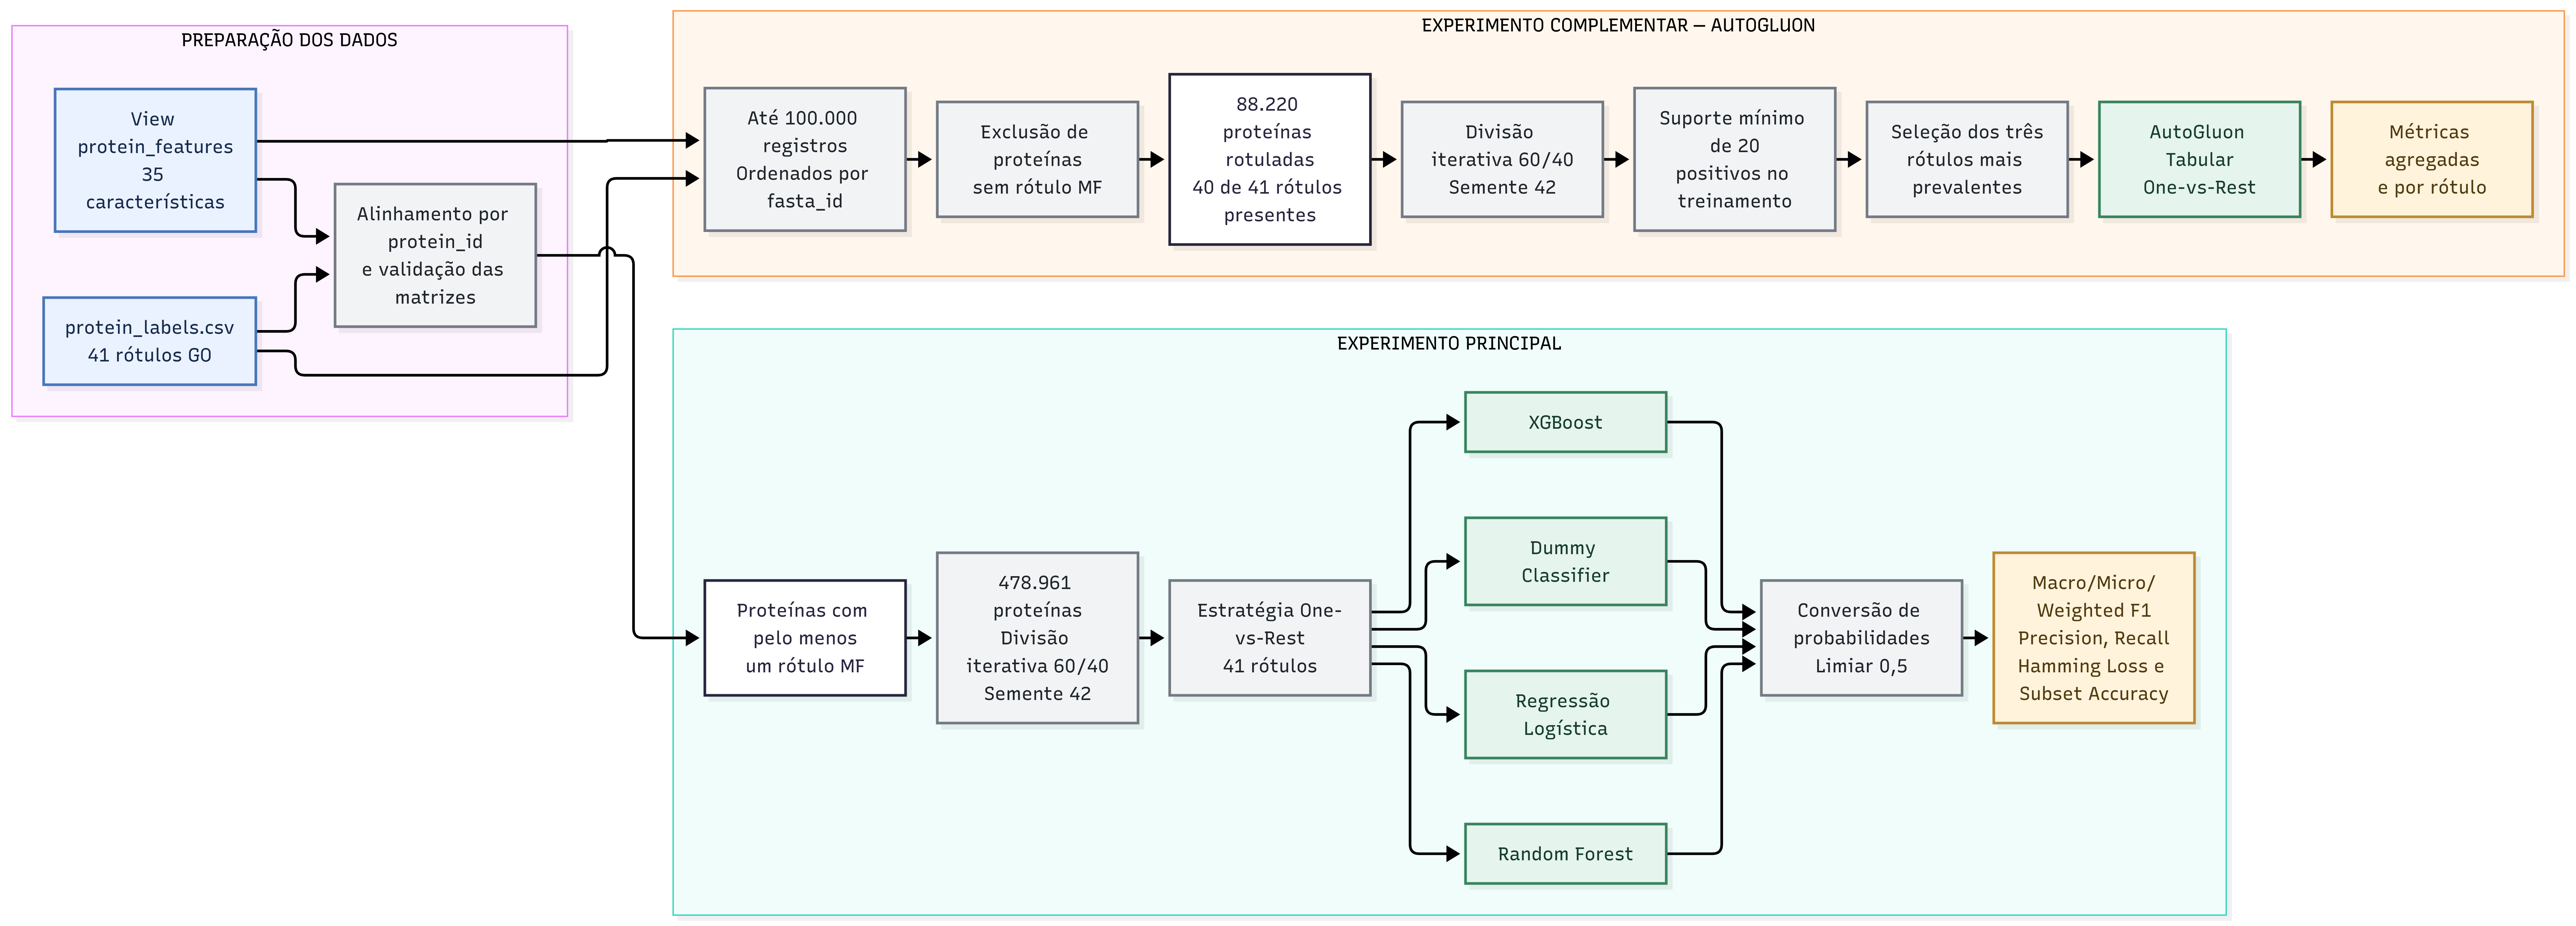
\includegraphics[width=\textwidth]
        {figuras/04-desenvolvimento/arquitetura-geral.png}
    \caption{Arquitetura geral do FASTA2GO.}
    \label{fig:arquitetura-geral}
    \legend{Fonte: Elaborado pelo autor (2026).}
\end{figure}

A persistência dos dados é realizada por meio do DuckDB, utilizado para armazenar as sequências e suas informações derivadas em estruturas relacionais. A tabela principal \texttt{proteins} mantém os registros de entrada, enquanto tabelas complementares armazenam características da sequência, composição de aminoácidos, composição de dipeptídeos, informações do UniProtKB e anotações GO.

Além das tabelas, o projeto utiliza views SQL para disponibilizar conjuntos de características já relacionados, evitando a duplicação de dados derivados. Entre elas, destaca-se a view \texttt{protein\_features}, utilizada para disponibilizar as características consumidas pelos notebooks de análise e modelagem.

A organização das principais entidades e seus relacionamentos está representada na \autoref{fig:modelo-relacional}.

\begin{figure}[htb]
    \centering
    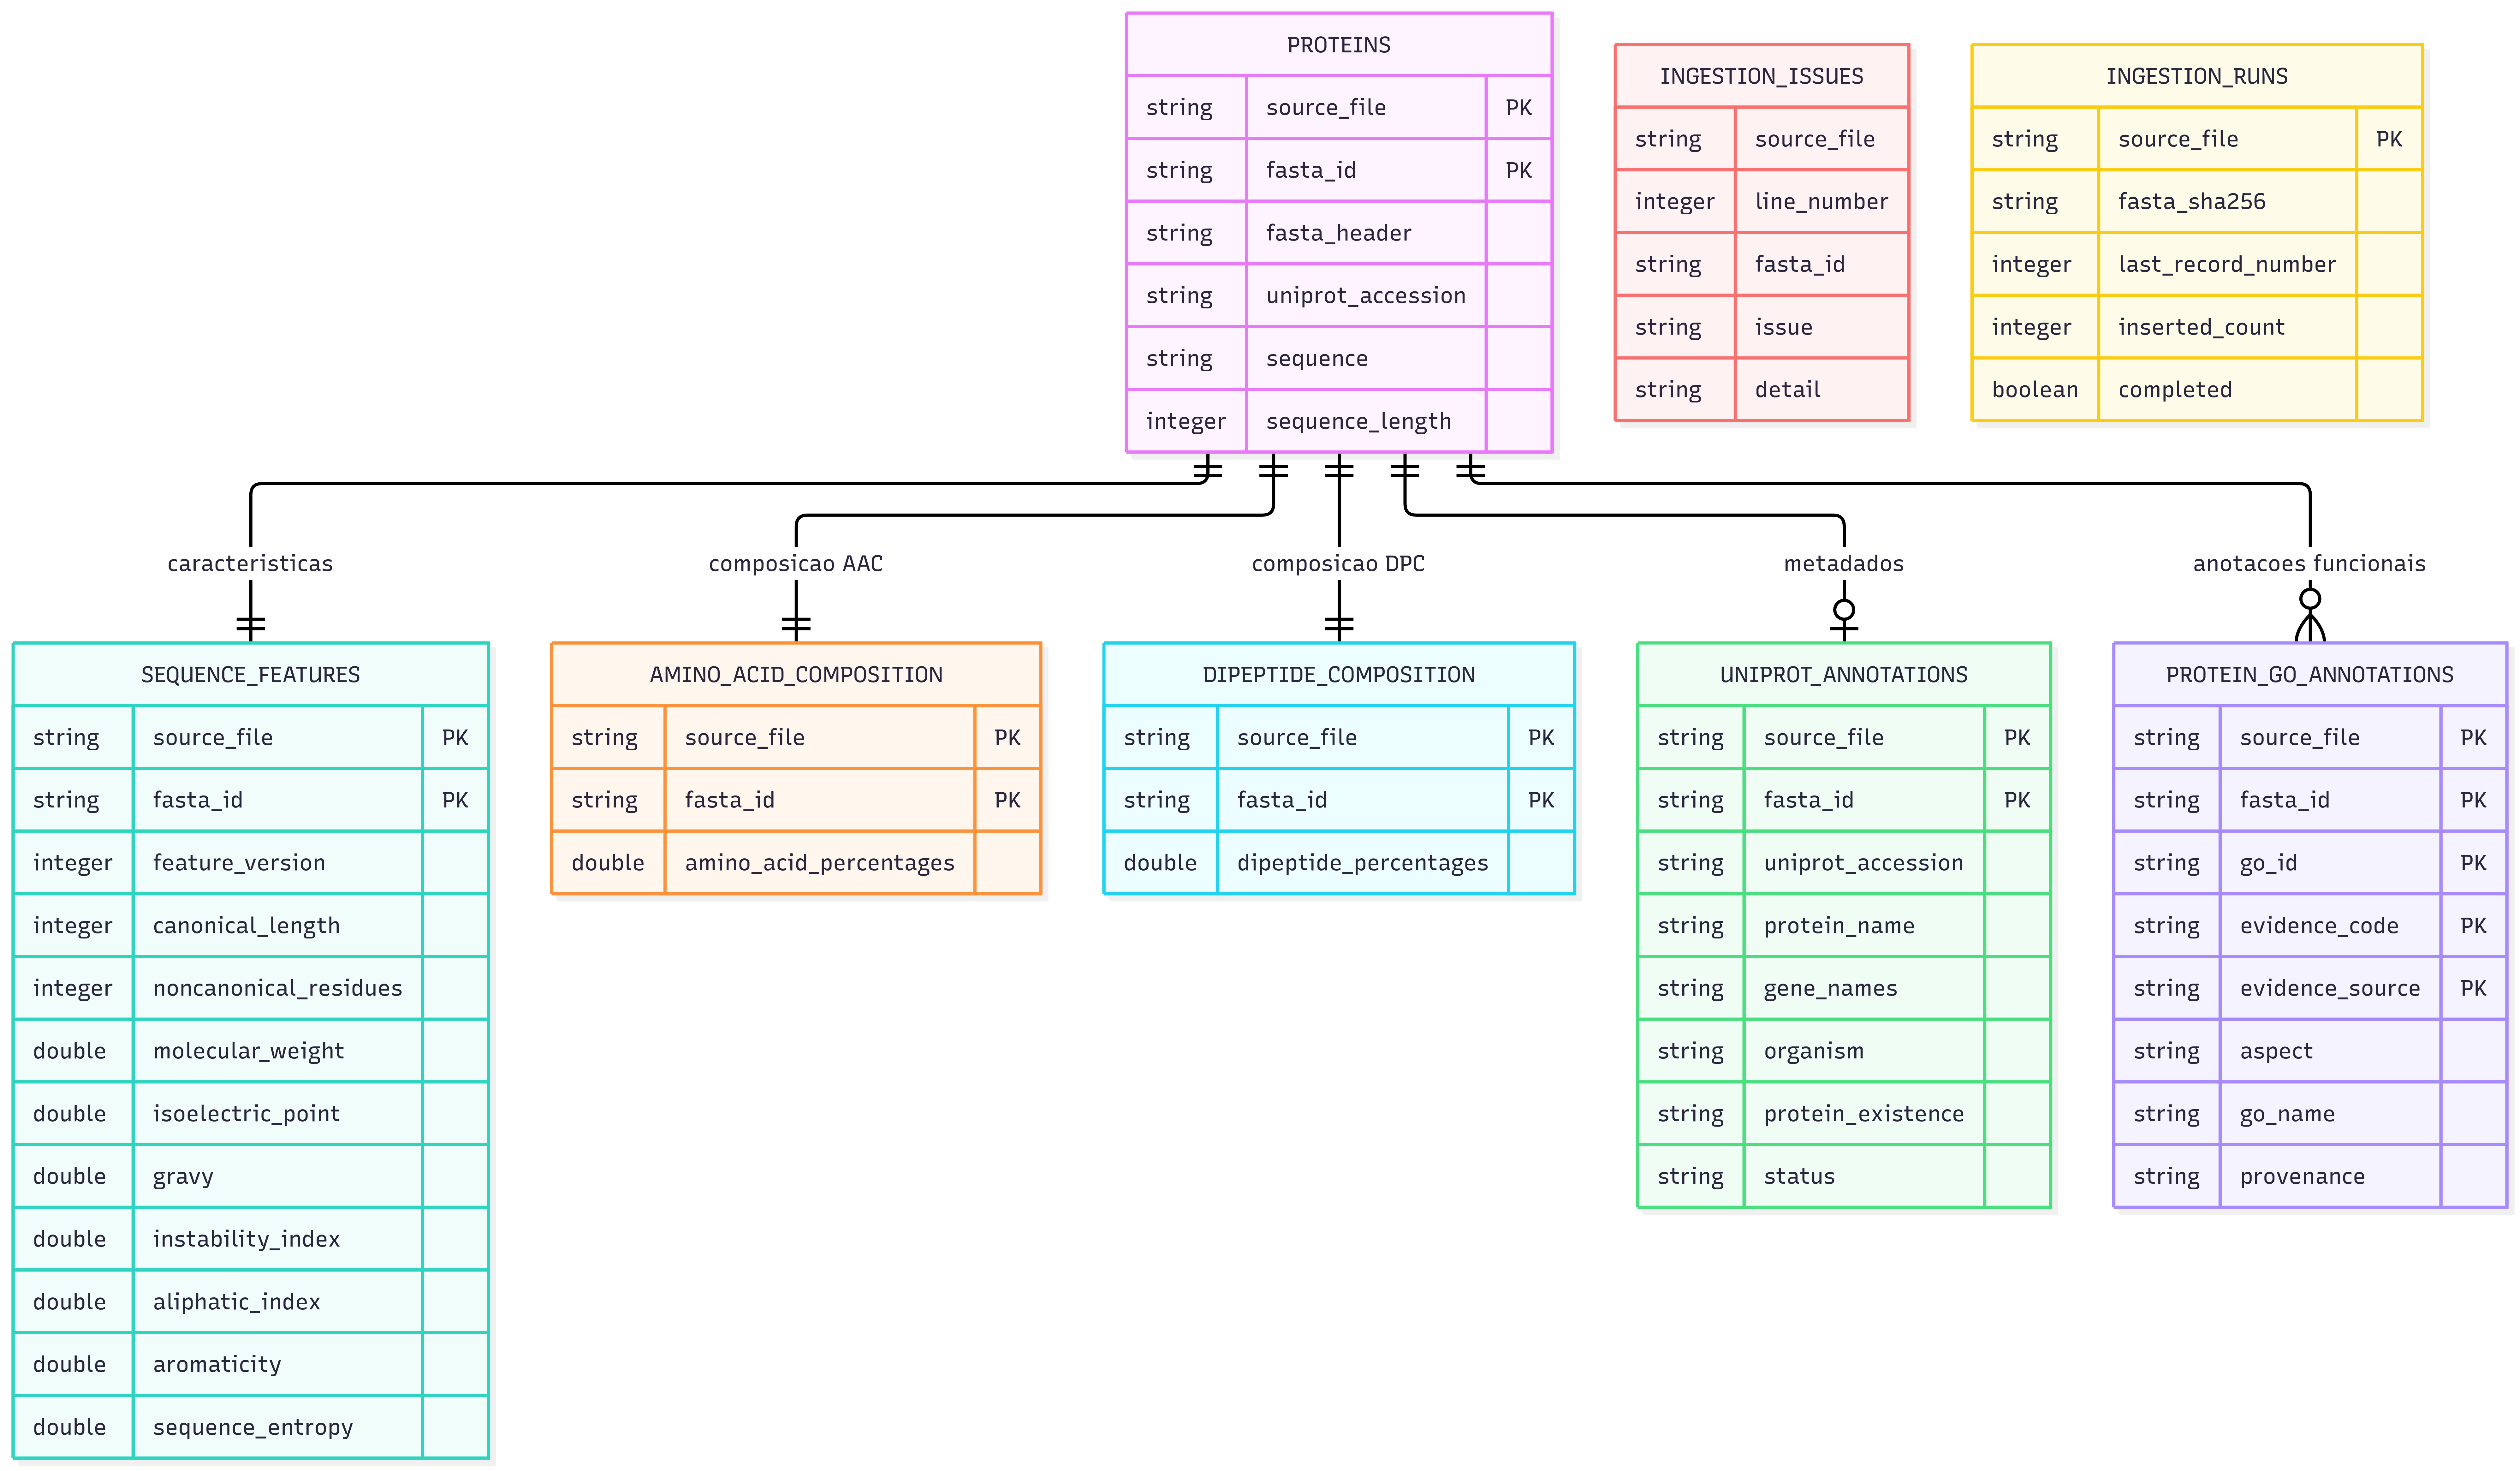
\includegraphics[width=\textwidth]
        {figuras/04-desenvolvimento/modelo-relacional.png}
    \caption{Modelo de dados utilizado pelo FASTA2GO.}
    \label{fig:modelo-relacional}
    \legend{Fonte: Elaborado pelo autor (2026).}
\end{figure}


%-------------------------------------------------------------------------------
% Implementação
%-------------------------------------------------------------------------------

\subsection{Implementação}
\label{sec:implementacao}

A implementação do FASTA2GO foi organizada em módulos Python e scripts SQL, responsáveis por funções específicas do pipeline. Essa separação permite executar individualmente as etapas de ingestão, construção dos rótulos, análise exploratória e modelagem, mantendo uma estrutura compartilhada para acesso e organização dos dados.

\subsubsection{Ingestão e armazenamento das sequências}

O processamento inicial é realizado por meio da leitura do arquivo FASTA em fluxo (\textit{streaming}), permitindo percorrer os registros sem carregar simultaneamente todo o arquivo em memória. Durante essa etapa, os cabeçalhos e identificadores são interpretados, as sequências são validadas e os registros são preparados para as operações posteriores.

As sequências são processadas em lotes de 5.000 registros. Para cada lote, são calculadas as características, consultadas as informações complementares do UniProtKB e preparados os dados para inserção no banco. As consultas ao UniProtKB são realizadas em blocos de até 200 identificadores de acesso por requisição.

A persistência utiliza transações para garantir que os registros de um lote sejam gravados de maneira consistente. O projeto também mantém informações de controle da ingestão, permitindo identificar o último lote confirmado e retomar o processamento após uma interrupção, desde que o arquivo de entrada e as configurações relevantes permaneçam inalterados.

Os registros que apresentam problemas de estrutura ou identificadores duplicados são documentados na tabela de ocorrências de ingestão. Sequências que possuem resíduos não canônicos são mantidas, mas esses resíduos são contabilizados separadamente para o tratamento adequado durante o cálculo das características.

\subsubsection{Extração das características}

A extração é implementada no módulo \texttt{features.py}, responsável por calcular propriedades físico-químicas, composição de aminoácidos e composição de dipeptídeos. Para o cálculo das características que exigem resíduos canônicos, são considerados os vinte aminoácidos convencionais.

Os resultados são armazenados em tabelas específicas. A composição de aminoácidos é representada por vinte percentuais, enquanto a composição de dipeptídeos contempla 400 combinações possíveis de pares adjacentes. As propriedades físico-químicas são armazenadas separadamente, permitindo que diferentes conjuntos de atributos sejam consultados posteriormente.

As sete classes químicas utilizadas nos experimentos são derivadas dos percentuais individuais dos aminoácidos por meio da view \texttt{protein\_features}. Dessa maneira, essas características não precisam ser armazenadas novamente como dados independentes.

Embora o sistema calcule e armazene as características DPC, os experimentos de modelagem utilizam um conjunto fixo de 35 atributos, composto por oito descritores físico-químicos e de sequência, vinte características AAC e sete classes químicas.

\subsubsection{Integração e rotulagem da Gene Ontology}

O enriquecimento funcional é realizado a partir das anotações associadas aos identificadores das proteínas no UniProtKB. Essas informações são armazenadas individualmente, preservando os termos GO, seus aspectos, códigos de evidência e informações de proveniência disponíveis.

A construção dos rótulos é realizada pelo módulo \texttt{go\_slim.py}, utilizando as fontes de ontologia e de definição do GO Slim fixadas no projeto. O processo relaciona as anotações originais ao vocabulário de 41 termos de Molecular Function, considerando as relações hierárquicas \texttt{is\_a} e \texttt{part\_of}.

Os identificadores alternativos são normalizados, termos obsoletos são rejeitados e as associações duplicadas são removidas. A propagação de ancestrais permite relacionar anotações específicas às categorias mais abrangentes contempladas pelo vocabulário. O resultado é exportado em formato CSV, com uma linha por proteína e seus respectivos rótulos funcionais.

O fluxo de construção dos rótulos é apresentado na \autoref{fig:fluxo-rotulagem-go}.

\begin{figure}[htb]
    \centering
    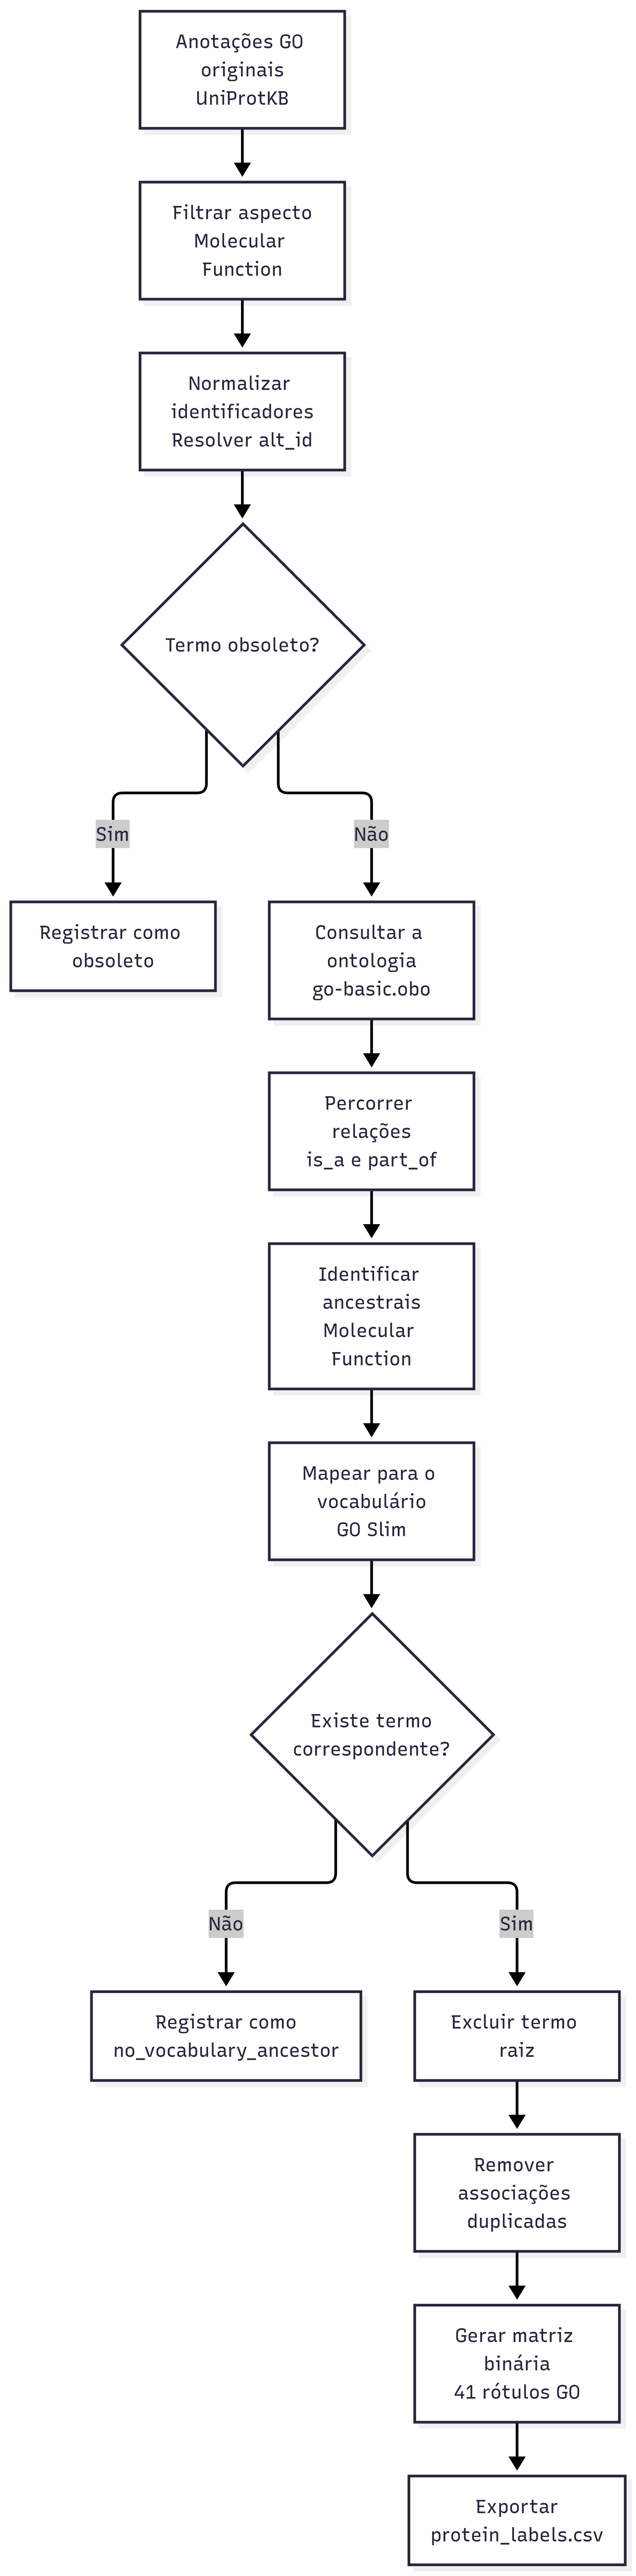
\includegraphics[width=0.85\textwidth]
        {figuras/04-desenvolvimento/fluxo-rotulagem-go.png}
    \caption{Fluxo de construção dos rótulos funcionais a partir da Gene Ontology.}
    \label{fig:fluxo-rotulagem-go}
    \legend{Fonte: Elaborado pelo autor (2026).}
\end{figure}

\subsubsection{Análise exploratória}

A análise exploratória é realizada no notebook \texttt{02\_analise\_exploratoria.ipynb}, que consulta a base DuckDB em modo somente leitura. Seu objetivo é verificar a integridade dos dados e investigar distribuições, correlações e possíveis redundâncias entre as características utilizadas.

São realizadas verificações de alinhamento entre tabelas, valores ausentes, consistência dos denominadores das frequências, distribuição das características e prevalência dos rótulos funcionais. Também são investigadas associações entre atributos e rótulos, permitindo identificar padrões que possam auxiliar na interpretação dos dados utilizados na modelagem.

Essa etapa não altera o banco de dados nem remove automaticamente características. As observações obtidas são utilizadas para documentar a estrutura da base e apoiar a interpretação dos experimentos posteriores. As visualizações selecionadas dessa análise são apresentadas na seção de resultados.

\subsubsection{Implementação dos experimentos de aprendizado de máquina}

A modelagem está organizada em dois notebooks. O primeiro, \texttt{03\_comparacao\_modelos.ipynb}, implementa a comparação entre Dummy Classifier, Regressão Logística, Random Forest e XGBoost. O segundo, \texttt{04\_predicao\_autogluon.ipynb}, executa um experimento complementar utilizando AutoGluon Tabular.

Nos dois casos, as características são obtidas a partir da view \texttt{protein\_features}, enquanto os rótulos são carregados do arquivo exportado durante a etapa de construção do GO Slim. A correspondência entre proteínas e rótulos é verificada por identificadores, garantindo o alinhamento entre as matrizes de entrada e saída.

A definição do conjunto de atributos utilizado na comparação principal é centralizada no notebook, conforme ilustrado pelo trecho de implementação a seguir:

\begin{lstlisting}[language=Python, caption={Definição do conjunto fixo de características}, label={lst:feature-columns}]
PHYSICOCHEMICAL = [
    "canonical_length", "molecular_weight", "isoelectric_point",
    "gravy", "instability_index", "aliphatic_index",
    "aromaticity", "sequence_entropy"
]

CHEMICAL_CLASSES = [
    "hydrophobic_pct", "polar_pct", "positive_pct",
    "negative_pct", "charged_pct", "aromatic_pct",
    "sulfur_pct"
]

FEATURE_COLUMNS = (
    PHYSICOCHEMICAL
    + features.AAC_COLUMNS
    + CHEMICAL_CLASSES
)

assert len(FEATURE_COLUMNS) == len(set(FEATURE_COLUMNS)) == 35
\end{lstlisting}

Na comparação principal, os quatro algoritmos são aplicados à mesma representação de entrada e aos mesmos subconjuntos de treinamento e teste. Cada modelo utiliza a estratégia One-vs-Rest para tratar os 41 rótulos funcionais, produzindo classificadores binários independentes.

O experimento complementar com AutoGluon utiliza a mesma representação de 35 características, mas mantém as configurações específicas de amostragem e seleção de rótulos definidas no notebook. Por essa razão, seus resultados são apresentados separadamente da comparação principal.

A sequência de preparação dos dados, treinamento e avaliação dos modelos está sintetizada na \autoref{fig:fluxo-experimentos}.

\begin{figure}[htb]
    \centering
    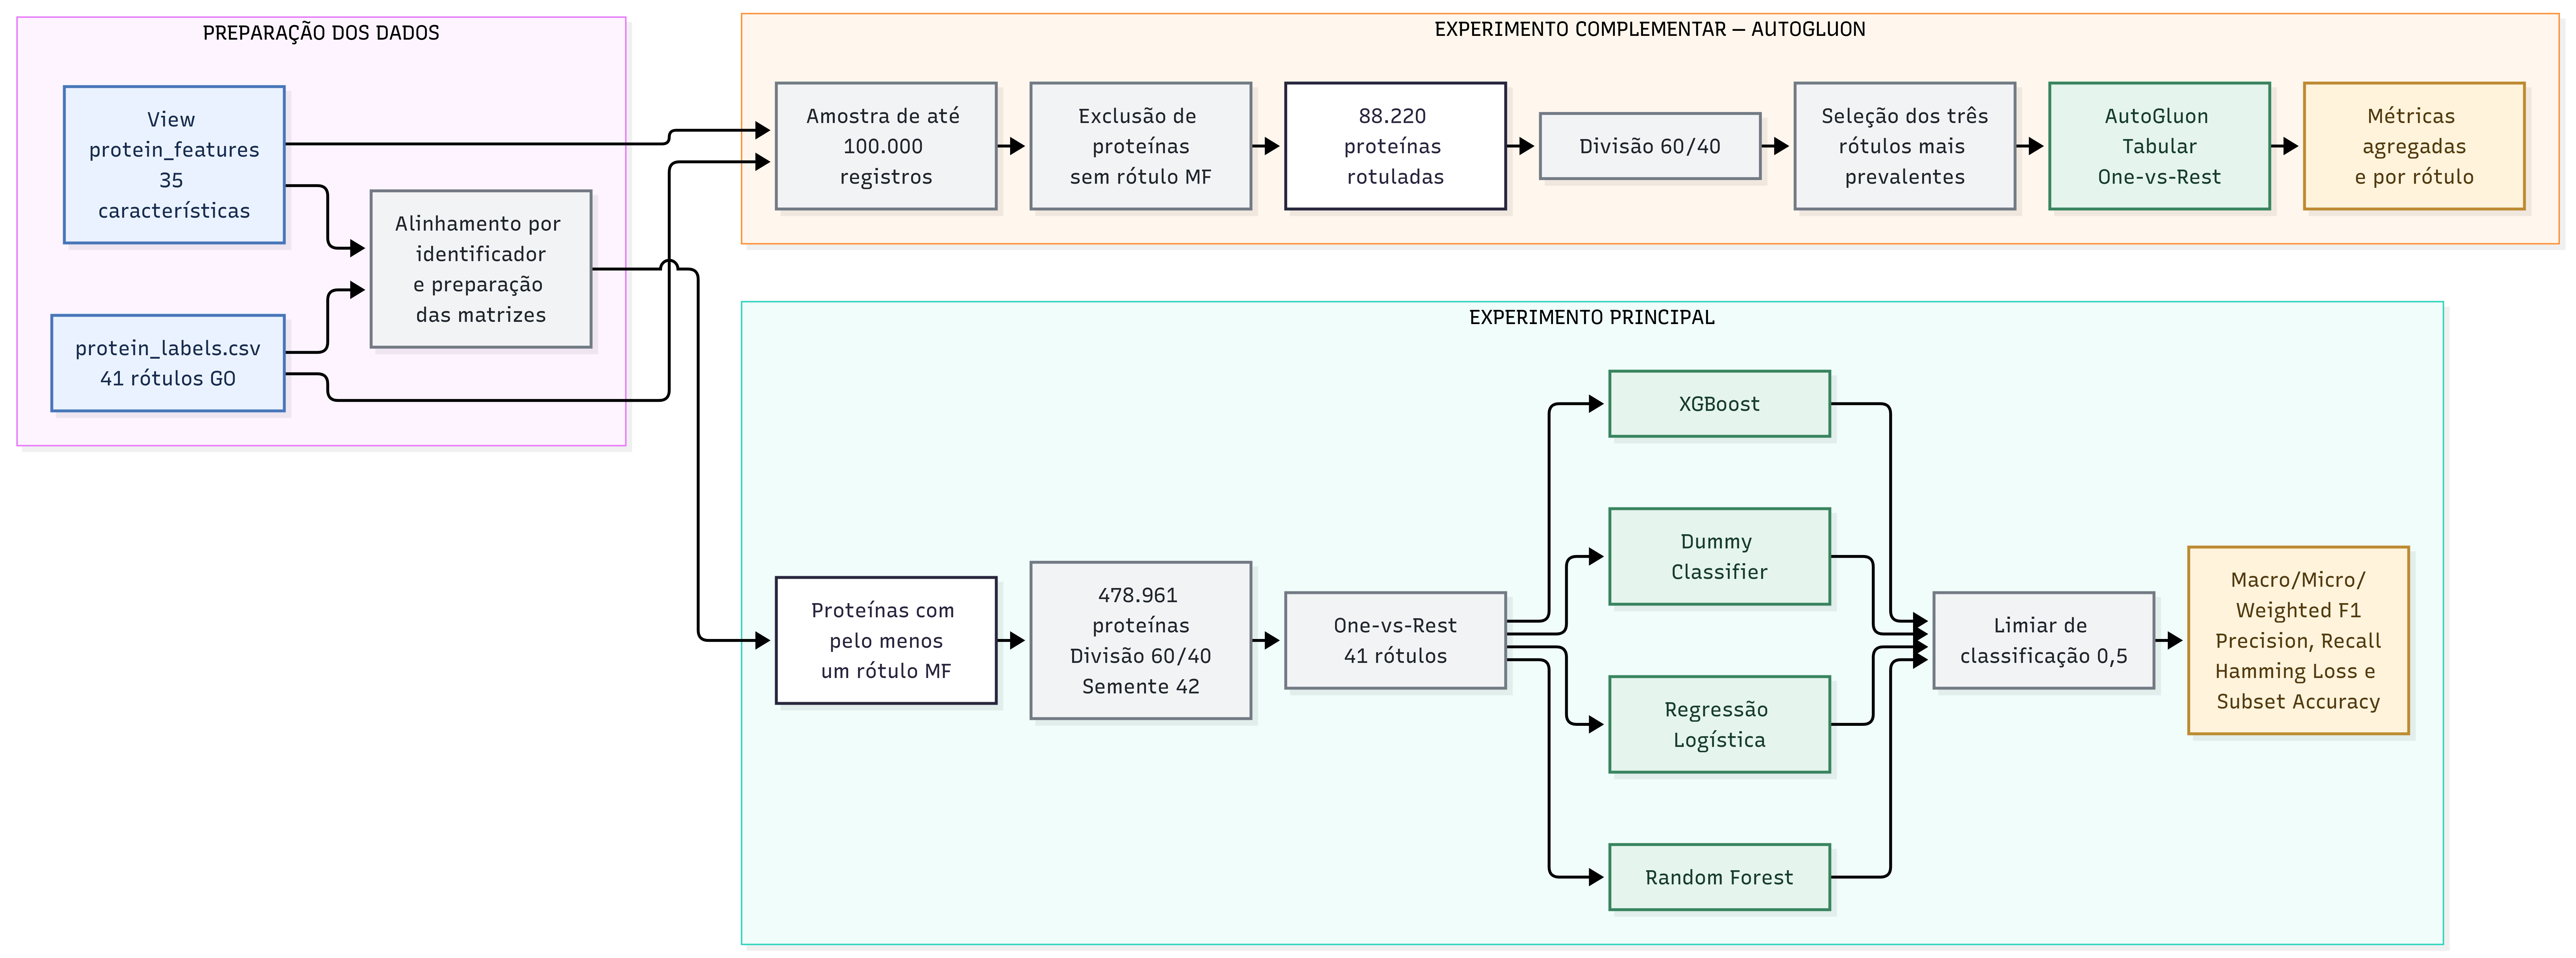
\includegraphics[width=0.90\textwidth]
        {figuras/04-desenvolvimento/fluxo-experimentos.png}
    \caption{Fluxo de preparação e execução dos experimentos de aprendizado de máquina.}
    \label{fig:fluxo-experimentos}
    \legend{Fonte: Elaborado pelo autor (2026).}
\end{figure}


%-------------------------------------------------------------------------------
% Resultados e Discussões
%-------------------------------------------------------------------------------

\subsection{Resultados e Discussões}
\label{sec:resultados-e-discussoes}

Os resultados são apresentados conforme as etapas de execução do FASTA2GO, começando pela integridade e organização dos dados, seguida das observações da análise exploratória e, por fim, da avaliação dos modelos de aprendizado de máquina.

\subsubsection{Resultados do processamento e organização dos dados}

A base utilizada pelo FASTA2GO contém 575.748 registros provenientes do UniProtKB/Swiss-Prot, totalizando 209.017.843 resíduos de aminoácidos. O comprimento médio das sequências é de aproximadamente 363 resíduos. Durante a ingestão, foram identificadas 2.685 sequências contendo resíduos não canônicos, que foram mantidas e sinalizadas para tratamento específico durante o cálculo das características.

As verificações de integridade registradas no projeto identificaram correspondência entre os registros de proteínas e suas respectivas tabelas de características, sem registros órfãos ou valores ausentes na view utilizada para os experimentos. A \autoref{tab:resultado-processamento} apresenta os principais indicadores obtidos.

\begin{table}[htb]
    \centering
    \ABNTEXfontereduzida
    \caption{Indicadores de processamento e integridade da base}
    \label{tab:resultado-processamento}
    \begin{tabular}{lr}
        \toprule
        \textbf{Indicador} & \textbf{Resultado} \\
        \midrule
        Registros FASTA & 575.748 \\
        Resíduos de aminoácidos & 209.017.843 \\
        Comprimento médio das sequências & 363 \\
        Sequências com resíduos não canônicos & 2.685 \\
        Registros na tabela de características & 575.748 \\
        Registros na composição AAC & 575.748 \\
        Registros na composição DPC & 575.748 \\
        Registros sem características associadas & 0 \\
        Anotações UniProtKB com correspondência & 575.748 \\
        \bottomrule
    \end{tabular}
    \legend{Fonte: Resultados registrados na validação da base FASTA2GO (2026).}
\end{table}

Na etapa de construção dos rótulos, foram processadas 1.088.243 anotações de função molecular. Desse total, 1.072.929 foram relacionadas a algum termo do vocabulário selecionado, correspondendo a 98,59\% das anotações processadas. Outras 14.946 não possuíam ancestral correspondente no vocabulário, enquanto 368 estavam associadas a termos obsoletos. Não foram identificados termos desconhecidos no processamento registrado.

Após a construção dos rótulos, 96.787 proteínas não apresentavam associação com os 41 termos de Molecular Function utilizados. Essas proteínas foram mantidas na base original, mas não foram incluídas nos experimentos de treinamento e teste. Assim, o conjunto experimental principal foi composto por 478.961 proteínas rotuladas.

\subsubsection{Resultados da análise exploratória}

A análise exploratória permitiu identificar características importantes da representação utilizada. Entre elas, destacam-se as distribuições assimétricas de comprimento, massa molecular e índice de instabilidade, além de relações de redundância entre alguns atributos.

Uma das redundâncias identificadas ocorre entre aromaticidade e percentual de aminoácidos aromáticos, pois representam a mesma proporção em escalas diferentes. Também foi observada uma correlação de aproximadamente 0,998 entre comprimento canônico e massa molecular.

Além disso, os vinte atributos de composição de aminoácidos somam 100\%, enquanto as sete classes químicas são calculadas como combinações desses mesmos percentuais. Essas dependências indicam que parte da informação presente nos atributos é compartilhada. Entretanto, o conjunto de 35 características foi mantido nos experimentos, conforme o escopo definido para a comparação dos algoritmos.

A \autoref{fig:correlacao-caracteristicas} apresenta a matriz de correlação entre as características utilizadas nos experimentos. Essa visualização permite observar as relações entre os atributos e identificar grupos de variáveis com comportamento semelhante.

\begin{figure}[htb]
    \centering
    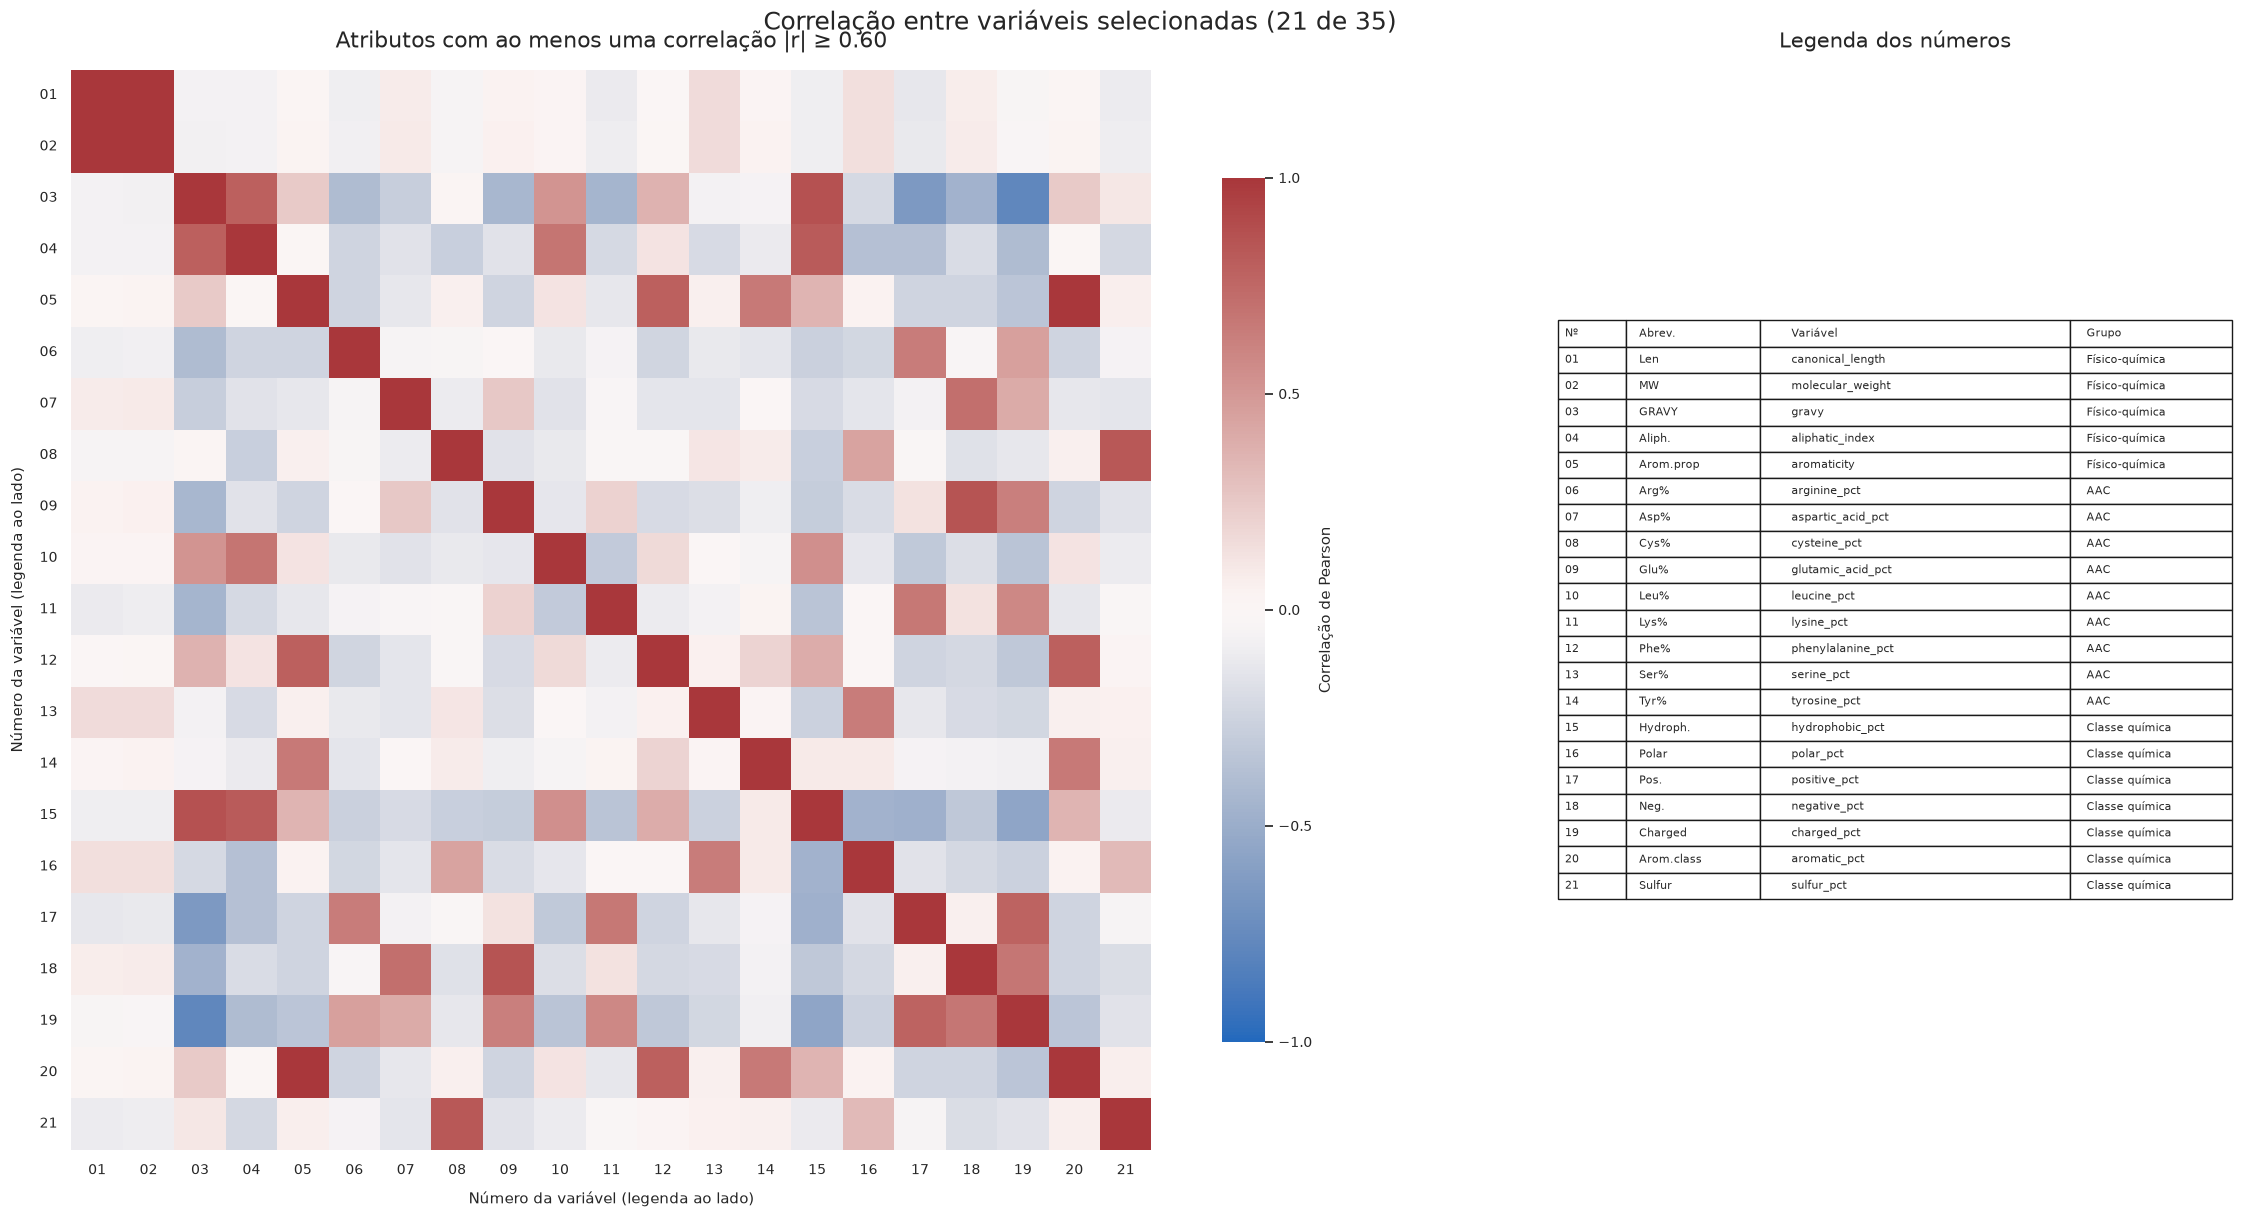
\includegraphics[width=\textwidth]
        {figuras/04-desenvolvimento/matriz_correlacao.png}
    \caption{Matriz de correlação entre as características utilizadas nos experimentos.}
    \label{fig:correlacao-caracteristicas}
    \legend{Fonte: Elaborado pelo autor a partir dos dados do FASTA2GO (2026).}
\end{figure}

A distribuição dos rótulos também merece atenção, uma vez que as funções moleculares apresentam frequências distintas na base. Essa característica pode afetar o treinamento e a avaliação dos modelos, especialmente nas métricas que atribuem o mesmo peso a cada categoria. A \autoref{fig:prevalencia-rotulos} apresenta a frequência das 41 categorias de Molecular Function consideradas no estudo.

\begin{figure}[htb]
    \centering
    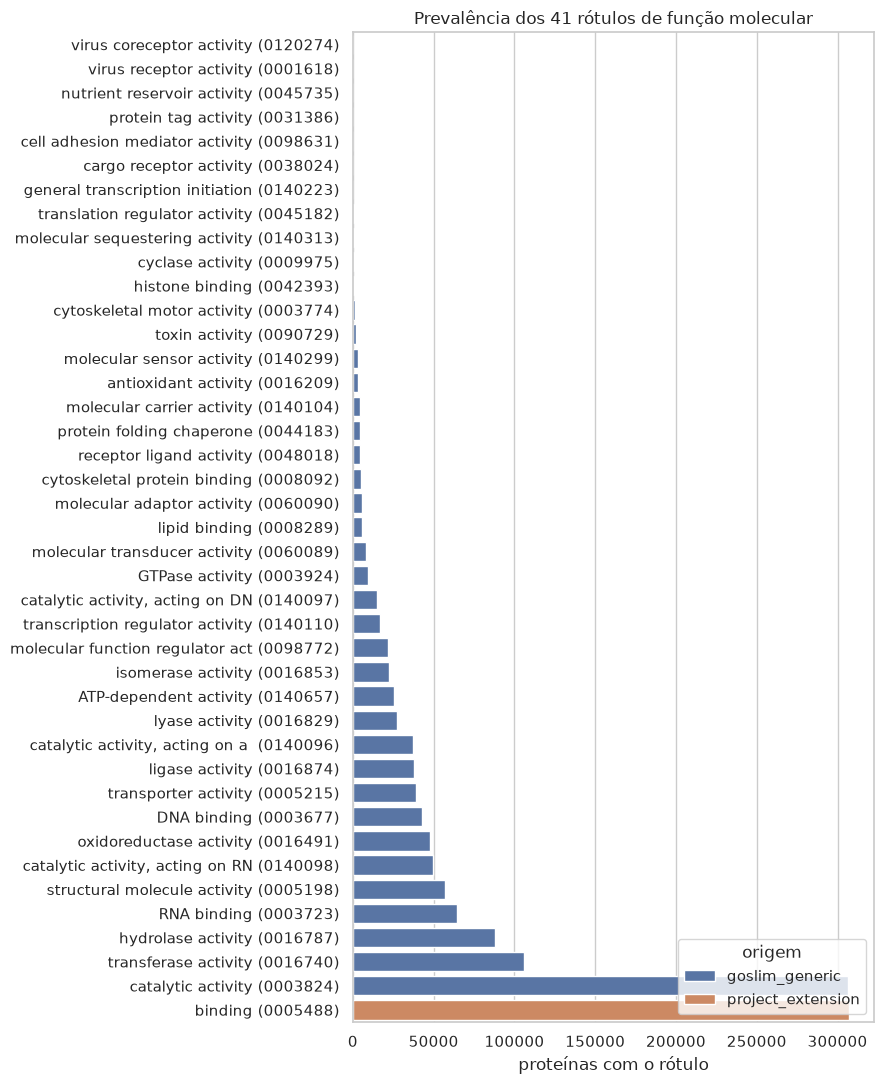
\includegraphics[width=\textwidth]
        {figuras/04-desenvolvimento/prevalencia-rotulos-go.png}
    \caption{Distribuição dos rótulos de Molecular Function utilizados na pesquisa.}
    \label{fig:prevalencia-rotulos}
    \legend{Fonte: Elaborado pelo autor a partir dos dados do FASTA2GO (2026).}
\end{figure}

\subsubsection{Resultados da comparação principal de algoritmos}

A comparação principal avaliou quatro algoritmos utilizando as mesmas 35 características, os mesmos 41 rótulos e a mesma divisão dos dados. Os resultados registrados para o conjunto de teste estão apresentados na \autoref{tab:resultados-modelos}.

\begin{table}[htb]
    \centering
    \ABNTEXfontereduzida
    \caption{Resultados da comparação principal dos modelos}
    \label{tab:resultados-modelos}
    \begin{tabular}{lrrrrr}
        \toprule
        \textbf{Modelo} & \textbf{Macro-F1} & \textbf{Micro-F1} &
        \textbf{Macro-Precision} & \textbf{Macro-Recall} & \textbf{Hamming Loss} \\
        \midrule
        Random Forest & 0,5430 & 0,8251 & 0,9463 & 0,4230 & 0,0220 \\
        XGBoost & 0,3468 & 0,6408 & 0,8748 & 0,2617 & 0,0416 \\
        Regressão Logística & 0,1343 & 0,5766 & 0,3463 & 0,1114 & 0,0485 \\
        Dummy Classifier & 0,0381 & 0,5267 & 0,0312 & 0,0488 & 0,0562 \\
        \bottomrule
    \end{tabular}
    \legend{Fonte: Resultados do notebook de comparação de modelos (2026).}
\end{table}

O Random Forest apresentou os melhores resultados entre os modelos da comparação principal, alcançando Macro-F1 de 0,5430, Micro-F1 de 0,8251 e Macro-Precision de 0,9463. O resultado indica que, nas condições experimentais avaliadas, o algoritmo apresentou o melhor desempenho geral entre os modelos comparados. Entretanto, seus resultados devem ser interpretados em conjunto com as demais métricas, especialmente a revocação.

Em particular, o Macro-Recall de 0,4230 do Random Forest indica que o modelo não recuperou uma parcela considerável dos exemplos positivos quando os rótulos são considerados individualmente. Dessa forma, a elevada precisão deve ser interpretada em conjunto com a revocação, pois uma quantidade menor de previsões positivas incorretas não significa necessariamente que todas as funções presentes foram identificadas.

O XGBoost apresentou o segundo melhor resultado em Macro-F1, com 0,3468, e Micro-F1 de 0,6408. Embora tenha obtido resultados inferiores aos do Random Forest, seu tempo de treinamento foi significativamente menor, aspecto relevante quando se considera o custo computacional dos experimentos.

A Regressão Logística apresentou desempenho inferior aos modelos baseados em árvores, especialmente na métrica Macro-F1. O Dummy Classifier, utilizado como referência, obteve o menor Macro-F1, demonstrando a limitação de uma estratégia baseada apenas nas prevalências observadas no conjunto de treinamento.

Além das métricas de classificação, os tempos de treinamento e predição foram registrados para cada modelo. Esses valores estão apresentados na \autoref{tab:tempos-modelos}.

\begin{table}[htb]
    \centering
    \ABNTEXfontereduzida
    \caption{Tempos de treinamento e predição dos modelos}
    \label{tab:tempos-modelos}
    \begin{tabular}{lrr}
        \toprule
        \textbf{Modelo} & \textbf{Treinamento (s)} & \textbf{Predição (s)} \\
        \midrule
        Random Forest & 8.228,59 & 278,53 \\
        XGBoost & 236,23 & 9,93 \\
        Regressão Logística & 115,59 & 0,58 \\
        Dummy Classifier & 1,55 & 0,18 \\
        \bottomrule
    \end{tabular}
    \legend{Fonte: Resultados do notebook de comparação de modelos (2026).}
\end{table}

Os tempos demonstram que o Random Forest apresentou o maior custo computacional entre os modelos avaliados. Seu tempo de treinamento foi consideravelmente superior ao do XGBoost, que obteve desempenho intermediário com menor tempo de execução. Esse resultado evidencia que a escolha de um algoritmo não deve considerar exclusivamente as métricas de classificação, mas também o custo necessário para sua execução.

A comparação visual das métricas de desempenho dos quatro algoritmos é apresentada na \autoref{fig:comparacao-modelos}.

\begin{figure}[htb]
    \centering
    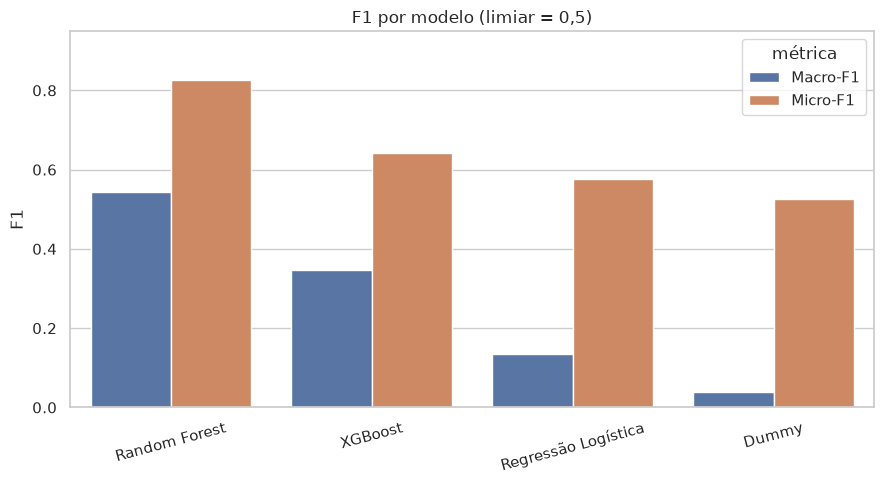
\includegraphics[width=0.95\textwidth]
        {figuras/04-desenvolvimento/comparacao-metricas-modelos.png}
    \caption{Comparação das métricas de desempenho dos modelos principais.}
    \label{fig:comparacao-modelos}
    \legend{Fonte: Elaborado pelo autor a partir dos resultados experimentais (2026).}
\end{figure}

Os resultados apresentados são descritivos de uma única divisão entre treinamento e teste. Portanto, não permitem afirmar significância estatística das diferenças observadas nem garantir generalização para proteínas sem relação de similaridade com aquelas presentes no treinamento. Essas limitações devem ser consideradas na interpretação dos resultados.

\subsubsection{Resultados do experimento complementar com AutoGluon}

O experimento complementar utilizou AutoGluon Tabular com sua configuração padrão definida no notebook. Foram considerados inicialmente 100.000 registros, dos quais 88.220 possuíam pelo menos um rótulo de Molecular Function. Nessa amostra, 40 dos 41 rótulos do vocabulário estavam presentes.

A configuração selecionou os três rótulos elegíveis mais prevalentes: atividade catalítica, atividade de ligação e atividade transferase. Os classificadores foram treinados individualmente pela estratégia One-vs-Rest, utilizando o mesmo conjunto de 35 características.

Os resultados agregados obtidos no conjunto de teste estão apresentados na \autoref{tab:resultados-autogluon}.

\begin{table}[htb]
    \centering
    \ABNTEXfontereduzida
    \caption{Resultados agregados do experimento com AutoGluon}
    \label{tab:resultados-autogluon}
    \begin{tabular}{lr}
        \toprule
        \textbf{Métrica} & \textbf{Resultado} \\
        \midrule
        Macro-F1 & 0,9004 \\
        Micro-F1 & 0,9243 \\
        Weighted-F1 & 0,9229 \\
        Macro-Precision & 0,9120 \\
        Macro-Recall & 0,8928 \\
        Hamming Loss & 0,0803 \\
        Subset Accuracy & 0,8040 \\
        \bottomrule
    \end{tabular}
    \legend{Fonte: Resultados do notebook de predição com AutoGluon (2026).}
\end{table}

A análise individual dos rótulos apresentou F1-score de 0,8172 para atividade transferase, 0,9197 para atividade de ligação e 0,9642 para atividade catalítica. Esses resultados demonstram que o desempenho variou entre as categorias consideradas, mesmo dentro de uma amostra reduzida e com seleção dos rótulos mais prevalentes.

Apesar dos valores agregados obtidos pelo AutoGluon serem superiores aos resultados da comparação principal, não é adequado concluir que essa ferramenta apresentou desempenho superior aos demais algoritmos. As condições experimentais são diferentes, pois o AutoGluon utilizou uma amostra de 100.000 registros e somente três rótulos, enquanto a comparação principal considerou 478.961 proteínas e 41 rótulos. Portanto, os resultados devem ser interpretados como um experimento complementar, e não como uma comparação direta entre todos os modelos.

A \autoref{fig:autogluon-rotulos} apresenta os valores de F1-score obtidos individualmente para os três rótulos avaliados com AutoGluon.

\begin{figure}[htb]
    \centering
    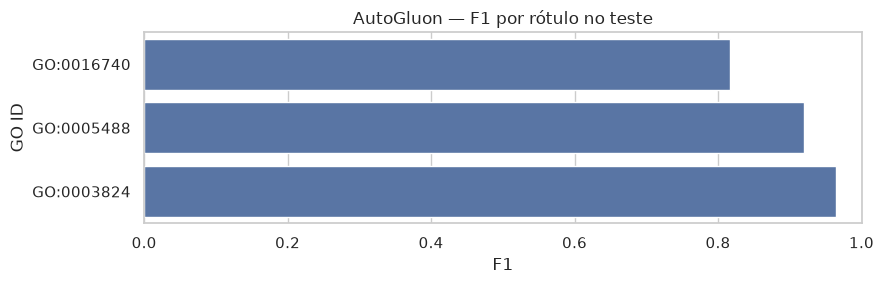
\includegraphics[width=0.85\textwidth]
        {figuras/04-desenvolvimento/f1-autogluon-por-rotulo.png}
    \caption{F1-score individual dos rótulos avaliados com AutoGluon.}
    \label{fig:autogluon-rotulos}
    \legend{Fonte: Elaborado pelo autor a partir dos resultados experimentais (2026).}
\end{figure}

\subsubsection{Síntese dos resultados}

Os experimentos demonstraram que diferentes algoritmos apresentam comportamentos distintos quando aplicados à predição multirrótulo de funções moleculares a partir de características de sequências proteicas. Na comparação principal, o Random Forest apresentou os maiores valores de Macro-F1, Micro-F1 e Macro-Precision, enquanto o XGBoost apresentou um compromisso diferente entre desempenho e tempo de execução.

O experimento complementar com AutoGluon apresentou resultados expressivos para os três rótulos selecionados, mas suas condições de execução impedem uma comparação direta com os modelos da análise principal.

Em conjunto, os resultados reforçam a importância de avaliar diferentes algoritmos em condições experimentais bem definidas. Também evidenciam limitações relacionadas à distribuição desigual dos rótulos, à redundância entre características e à utilização de uma única divisão dos dados. Assim, a interpretação dos resultados deve permanecer restrita ao conjunto de dados, às características e às configurações efetivamente avaliadas.